\section{Atom-field interaction. Semiclassical theory}
\label{sec:atom-field_interaction}

The word \textit{semiclassical} in this context means the following: let us consider a classical electromagnetic field and a "quantum" atom. For simplicity let us take the two-level system (fig. \ref{fig:2lvl}). Then throw light on this system.
\begin{figure}[h!]
	\centering
	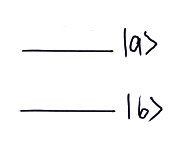
\includegraphics[width=0.35\linewidth]{fig/L4/2lvl}
	\caption{Atom's energy levels }
	\label{fig:2lvl}
\end{figure}

Mr. Hamiltonian is given by
\begin{equation}
	\hat{\mathscr{H}} = \frac{\hat{\vec{p}}^2}{2 m} + \hat{V} (\vec{r}).
\end{equation}
System has eigenstates which are given by equation
\begin{equation}
	\hat{\mathscr{H}} \ket{\psi} = E \ket{\psi}.
\end{equation}
So we have $E_a$ for $\ket{a}$ and $E_b$ for $\ket{b}$. After introducing electromagnetic field we have
\begin{equation}
	\hat{\mathscr{H}} = \frac{(\hat{\vec{p}} - \frac{e}{c} \vec{A})^2}{2m} + \hat{V}(\vec{r}) + e \varphi.
\end{equation}
Potentials are not determined and gauge transformation may take place:
\begin{equation}
	\vec{A} \to \vec{A} + \frac{\hbar c}{e} \nabla \chi, \qquad \varphi \to \varphi - \frac{\hbar c}{e} \parder{\chi}{t}.
\end{equation}
and
\begin{equation}
	\psi \to \psi e^{i \chi(\vec{r},t)}.
\end{equation}

Let a plane wave is falling 
\begin{equation}
	\vec{A} = \vec{A}_0 e^{i \vec{k}\vec{r} - i \omega t} = \vec{A}_0(t) e^{i \vec{k}\vec{r}}.
\end{equation}
Assume that characteristic scale of the system is such that 
\begin{equation}
	L \ll \lambda
	\label{eq:condition}
\end{equation}
is satisfied. Condition \eqref{eq:condition} is satisfied for lots of quantum systems. 
For example, visible light is $\lambda \sim 400 \div 800 \text{ nm}$, 
characteristic size of an atom is about $10^{-10} \text{ m}$, size of a quantum dot is about $10 \text{ nm}$. 

\begin{figure}[h!]
	\centering
	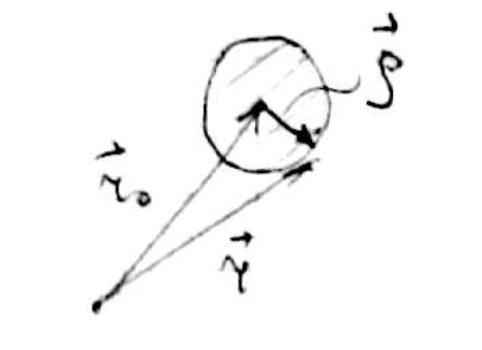
\includegraphics[width=0.3\linewidth]{fig/L4/simply}
	\caption{System}
	\label{fig:simply}
\end{figure}


Using this simplification we can $\vec{r}_0 \to \vec{r}$, where $\vec{r}_0$ is a vector of a centre of the system. This result may be achieved more formally by expanding $\vec{A}$ near $\vec{r}_0$ in Taylor series:
\begin{equation}
	\vec{A} (\vec{r},t) \approx \vec{A}_0 (t) e^{i \vec{k} \vec{r}_0} \left( 1 + i \vec{k} \bm{\rho} \right) \approx \vec{A}_0 e^{i \vec{k} \vec{r}_0}.
\end{equation} 
So field does not change in space, but in time. Let us choose the system of axes so as to $\vec{r}_0 = 0$. It means that $\vec{A} \approx \vec{A}_0 (t)$. So
\begin{equation}
	\hat{\mathscr{H}} = \frac{1}{2m} \left( \hat{\vec{p}}  - \frac{e}{c} \vec{A}_0(t) \right)^2 + V (\vec{r}) + e \varphi.
\end{equation}
The standard choice it to use Coulomb gauge:
\begin{equation}
	\Div \vec{A} = 0, \qquad \varphi = 0.
\end{equation}
After that, using $\hat{\vec{p}} = -i \hbar \nabla$, we obtain
\begin{equation}
	\hat{\mathscr{H}} = - \frac{\hbar^2}{2m} \left( \nabla - \frac{i e}{\hbar c} \vec{A}_0  \right)^2 + V(\vec{r}).
\end{equation}
Lets introduce a new wave function $\widetilde{\psi} = \psi \underbrace{e^{- i \frac{e}{c \hbar} \vec{A}_0 \vec{r}}}_{\hookrightarrow = u}$. After that, the $ u^{\dagger} \hat{\mathscr{H}} u $ transformation will make an impulse shift.
\begin{equation}
	\hat{\mathscr{H}} \psi = \hat{\mathscr{H}} \widetilde{\psi} e^{i \frac{e}{c \hbar} \vec{A}_0 (t) \vec{r}}.
\end{equation}
We shall call $\vec{g} \myeq \frac{e}{c \hbar} \vec{A}_0 (t)$. After that lets consider
\begin{equation}
	\left( \nabla - i \vec{g} \right) \left( \nabla - i \vec{g} \right) \widetilde{\psi} e^{i \vec{g} \vec{r}} = \\ = \left( \nabla - i \vec{g} \right) \left( \nabla \widetilde{\psi}  \right) e^{i \vec{g} \vec{r}} = \left( \nabla^2 \widetilde{\psi} \right) e^{i \vec{g} \vec{r}}.
\end{equation}
Schroedinger equation gives us
\begin{equation}
	\hat{\mathscr{H}} \psi = i \hbar \parder{\psi}{t},
\end{equation}
\begin{equation}
	\underbrace{\left( - \frac{\hbar^2}{2m} \nabla^2 + V \right)}_{\hat{\mathscr{H}}_0} \widetilde{\psi} (\vec{r},t) = i \hbar \parder{\widetilde{\psi}}{t} - \hbar \vec{r} \cdot \parder{\vec{g}}{t} \widetilde{\psi}.
	\label{eq:tmp143}
\end{equation} 
Lets pay attention to  
\begin{equation}
	\parder{\vec{g}}{t} = \frac{e}{\hbar c} \parder{\vec{A}_0(t)}{t} = - \frac{e}{\hbar} \vec{E}(t).
\end{equation}
Using that we can rewrite \eqref{eq:tmp143} as
\begin{equation}
	\hat{\mathscr{H}}_0 \widetilde{\psi} - e \vec{r} \vec{E} \widetilde{\psi} = i \hbar \parder{\widetilde{\psi}}{t}.
\end{equation}
It's convenient to denote $\hat{\mathscr{H}}_1 \myeq - e \vec{r} \vec{E}$ --- a dipole energy in electric field, so finally
\begin{equation}
	\left( \hat{\mathscr{H}}_0 + \hat{\mathscr{H}}_1 \right) \widetilde{\psi} = i \hbar \parder{\widetilde{\psi}}{t}.
\end{equation}

Let us do an expansion of $\psi$ in eigenstates:
\begin{equation}
	\ket{\psi} = C_a(t) \ket{a} + C_b(t) \ket{b},
\end{equation}
where
\begin{equation}
	\hat{\mathscr{H}}_0 \ket{a} = E_a \ket{a}, \qquad \hat{\mathscr{H}}_0 \ket{b} = E_b \ket{b}.
\end{equation}
Beside $E_a - E_b = \hbar \omega_0$ --- the transition frequency. Let incident field be $\bm{\varepsilon} = \bm{\varepsilon}_0 \cos \omega t$, so $\hat{\mathscr{H}}_1 = - \vec{d} \cdot \bm{\varepsilon}$. Let define initial conditions at moment $t = 0$:
\begin{equation}
	\ket{\psi} \Big|_{t = 0} = \ket{b} \qquad \to \qquad
	\begin{matrix}
		C_a(0) = 0, \\
		C_b(0) = 1.
	\end{matrix}
\end{equation}
So solution is
\begin{equation}
	\left( E_a C_a \ket{a} + E_b C_b \ket{b} \right) - \vec{d} \cdot \bm{\varepsilon} C_a \ket{a} - \vec{d} \cdot \bm{\varepsilon} C_b \ket{b} = i \hbar \dot{C}_a \ket{a} + i \hbar \dot{C}_b \ket{b}.
	\label{eq:tmp150}
\end{equation}
Projections to $\ket{a}$ and $\ket{b}$ gives us 
\begin{equation}
\begin{cases}
	\begin{matrix}
	\bra{a} \cdot \eqref{eq:tmp150}: &\qquad&
	E_a C_a - C_a \bra{a} \vec{d} \cdot \bm{\varepsilon} \ket{a} - C_b \bra{a} \vec{d} \cdot \bm{\varepsilon} \ket{b} = i \hbar \dot{C}_a, \\  \\
	\bra{b} \cdot \eqref{eq:tmp150}: &\qquad& 
	E_b C_b - C_b \bra{b} \vec{d} \cdot \bm{\varepsilon} \ket{b} - C_a \bra{b} \vec{d} \cdot \bm{\varepsilon} \ket{a} = i \hbar \dot{C}_b.
	\end{matrix}
\end{cases}
\label{eq:tmp151}
\end{equation}

Let us assume that field $\bm{\varepsilon}$ is not changing in space, so we can write
\begin{equation}
	\bra{a} \vec{d} \cdot \bm{\varepsilon} \ket{a} = \bra{a} \vec{d} \ket{a} \cdot \bm{\varepsilon}, \qquad 
	\bra{a} \vec{d} \cdot \bm{\varepsilon} \ket{b} = \bra{a} \vec{d} \ket{b} \cdot \bm{\varepsilon}.
\end{equation}
Dipole matrix elements are
\begin{equation}
	\vec{d}_{\alpha \beta} \myeq \bra{\alpha} \vec{d} \ket{\beta} = \int dV \psi_{\alpha}^* (\vec{r}) e \vec{r} \psi_{\beta} (\vec{r}).
\end{equation}
By symmetry considerations it follows  $\left| \vec{d}_{\alpha \alpha} \right| \ll \left| \vec{d}_{\alpha \beta} \right|_{\alpha \neq \beta}$, since usually neighboring states have opposite parity \textcolor{red}{(no eto ne tochno)} and $e \vec{r}$ --- an odd function. Using such approximation (formally just $\vec{d}_{aa}, \vec{d}_{bb} \to 0$ in \eqref{eq:tmp151}) we can write
\begin{equation}
	\begin{cases}
		i \hbar \dot{C}_a = E_a C_a - C_b \vec{d}_{ab} \cdot \bm{\varepsilon}, \\
		i \hbar \dot{C}_b = E_b C_b - C_a \vec{d}_{ba} \cdot \bm{\varepsilon}.
	\end{cases} 
	\qquad \quad \vec{d}_{ba} = \vec{d}_{ab}^*
\end{equation}
Here we can see that if we <<turn off>> the interaction ($\vec{d}_{\alpha \beta} = 0$) states $\ket{a}$ and $\ket{b}$ will be unloosened. If we turn the interaction on transitions will take place. 

To get rid off phase factor we introduce
\begin{equation}
	\widetilde{C}_a (t) \myeq C_a(t) e^{\frac{i}{\hbar}E_a t}, \qquad \widetilde{C}_b (t) \myeq C_b(t) e^{\frac{i}{\hbar}E_bt}.
\end{equation}
After that we have
\begin{equation}
	\begin{cases}
		\dot{\widetilde{C}}_a = \frac{i}{\hbar}\vec{d}_{ab} \cdot \bm{\varepsilon} e^{i \omega_0 t} \widetilde{C}_b(t), \\
		\dot{\widetilde{C}}_b = \frac{i}{\hbar}\vec{d}^*_{ab} \cdot \bm{\varepsilon} e^{-i \omega_0 t} \widetilde{C}_a(t).
	\end{cases} 
\end{equation}

Now we need to apply \textit{rotating wave approximation} (RWA). To understand what is it lets look at 
\begin{equation}
	\bm{\varepsilon}(t) e^{i \omega_0 t} = \bm{\varepsilon}_0 \frac{e^{i \omega t} + e^{- i \omega t}}{2} e^{i \omega_0 t}= \frac{1}{2} \bm{\varepsilon}_0 \left( \underbrace{e^{i(\omega_0 + \omega) t}}_{\text{fast osc.}} + e^{i(\omega_0 - \omega) t} \right).
\end{equation}
Fast oscillating term will lead to a small contribution, so it may be neglected. Leaving only $\sim e^{i (\omega_0 - \omega)t}$ term is called RWA. It's convenient to denote $\Delta \myeq \omega_0 - \omega$, so
\begin{equation}
	\begin{cases}
		\dot{\widetilde{C}}_a = \frac{i}{2\hbar}\vec{d}_{ab} \cdot \bm{\varepsilon}_0 e^{i \Delta t} \widetilde{C}_b(t), \\
		\dot{\widetilde{C}}_b = \frac{i}{2\hbar}\vec{d}^*_{ab} \cdot \bm{\varepsilon}_0 e^{-i \Delta t} \widetilde{C}_a(t).
	\end{cases} 
\end{equation}
Agreed notation is the following
\begin{equation}
	\boxed{\Omega_R \myeq \frac{\left|\vec{d}_{ab} \cdot \bm{\varepsilon}_0\right|}{\hbar}.}
\end{equation}
This is \textit{Rabi frequency}.

To simplify the understanding of our result let us put $\Delta =0$ (resonant excitation) and a specific phase of incident light, so our system will be
\begin{equation}
	\begin{cases}
		\dot{\widetilde{C}}_a = i \frac{\Omega_R}{2} \widetilde{C}_b, \\
		\dot{\widetilde{C}}_b = i \frac{\Omega_R}{2} \widetilde{C}_a.
	\end{cases}
	\label{eq:rabi_system}
\end{equation}
The solution is easy to obtain: $\widetilde{C}_b = \cos \left( \frac{\Omega_R t}{2} \right)$. Only $\left| C_a\right|^2$ and $\left| C_b \right|^2$ have the real physical meaning --- it's the probability of occupation on different states.
\begin{figure}[h!]
	\centering
	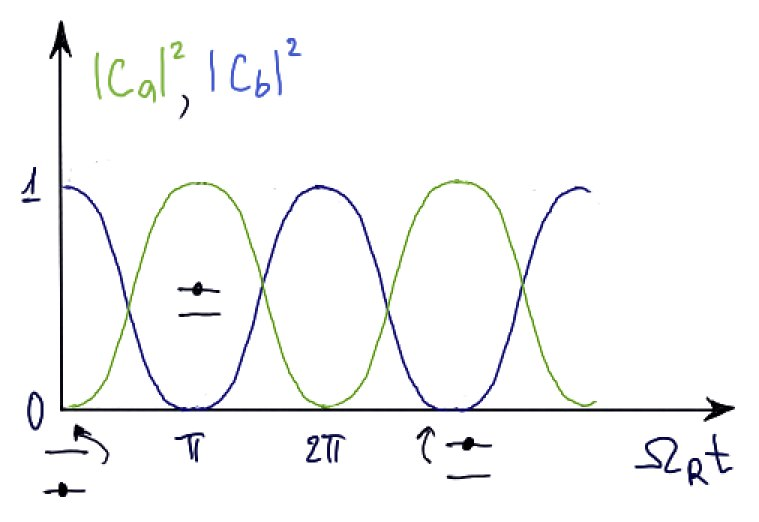
\includegraphics[width=0.65\linewidth]{fig/L4/rabi_osc}
	\caption{Rabi oscillations for two-level system}
	\label{fig:rabiosc}
\end{figure}

Here is a short summary:
\begin{enumerate}
	\item If $\vec{d} \perp \bm{\varepsilon}$ then $\Omega_R = 0$.
	\item To increase Rabi frequency one need to increase the amplitude of incident wave $\left| \bm{\varepsilon} \right|$. 
\end{enumerate}
